%!TEX root = ../thesis.tex

\subsection{結果}

各アルゴリズムのDAGの推定精度を図\ref{fig:plot_gaussian}
と\ref{fig:plot_uniform}に示す。
図\ref{fig:plot_gaussian}は
連続変数の誤差変数が正規分布に従うように生成したデータにおける推定精度を、
図\ref{fig:plot_uniform}は一様分布に従うように生成したデータにおける推定精度を示す。

実験結果より、提案アルゴリズムは他のアルゴリズムと比較して適合率も再現率も高いことが分かる。
また、提案アルゴリズムは他のアルゴリズムと比較して、サンプルサイズが大きくなるほど
有向辺の向きを正しく推定していることが分かる。
このことから、提案モデルは識別可能であり、本論文による提案アルゴリズムによって推定可能であると言える。
一方、DirectLiNGAMの推定精度は、正規分布の場合は適合率も再現率も0.5を下回るのに対し、
一様分布の場合はGESやMMHCの精度と同程度またはそれ以上である。
これは、LiNGAM\cite{Shimizu2011-pd}が誤差変数に対して非正規性を
仮定していることが影響しているためであると考えられる。

提案アルゴリズムにおける適合率と再現率を比較すると、
サンプルサイズが1000を超えると再現率のほうが高いことが読み取れる。
つまり、サンプルサイズが大きい時、
実際には直接的な因果関係があるにもかかわらず因果関係が無いと推定してしまうという偽陰性が少ない
ことを示している。
因果関係に関する仮説を得ようとする際に偽陽性が多いと、
重要な因果関係を見過ごしてしまう可能性が高まる。
そのため、因果関係の仮説を構築する上で、提案アルゴリズムの再現率が高いことは望ましいと言える。

\begin{figure}[H]
  \centering
  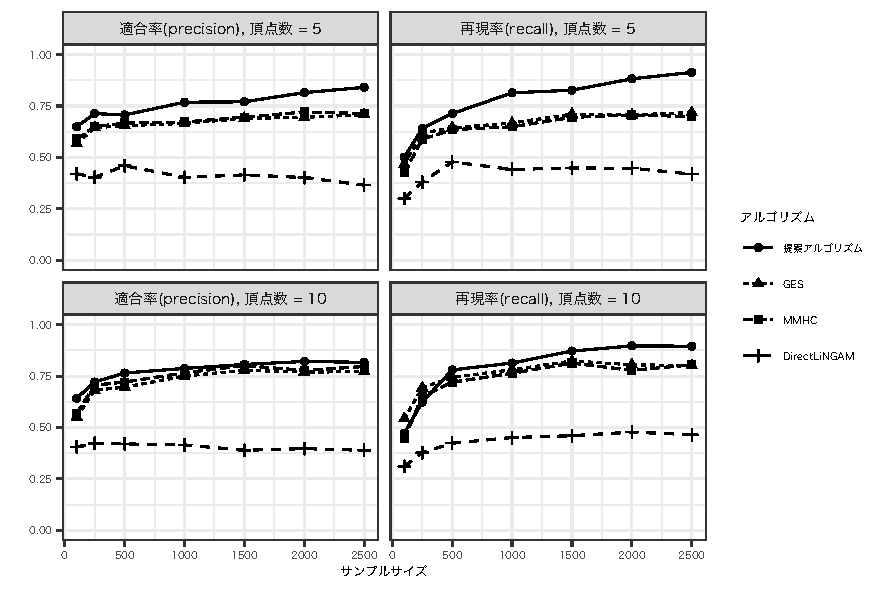
\includegraphics[width=13cm, bb=9 9 358 434]{./picture/plot_gaussian.pdf}
  \caption{連続変数の誤差変数が正規分布に従う提案モデルにおける各アルゴリズムの精度比較}
  \label{fig:plot_gaussian}
\end{figure}

\begin{figure}[H]
  \centering
  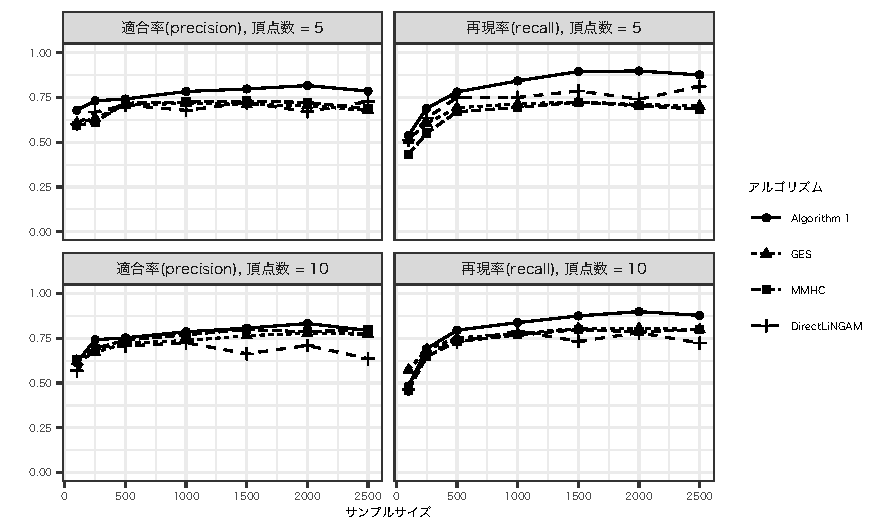
\includegraphics[width=13cm, bb=9 9 358 434]{./picture/plot_uniform.pdf}
  \caption{連続変数の誤差変数が一様分布に従う提案モデルにおける各アルゴリズムの精度比較}
  \label{fig:plot_uniform}
\end{figure}
